\documentclass{article}

\usepackage[T1]{fontenc}
\usepackage[utf8]{inputenc}
\usepackage{lmodern}
\usepackage[a4paper, bottom=4cm]{geometry} % bottom margin decreased
\usepackage{amsmath}
\usepackage{amssymb}
\usepackage{subfiles} % Best loaded last in the preamble
\usepackage{graphicx, caption}
\usepackage{color, xcolor}   %May be necessary if you want to color links
\usepackage{hyperref}
\usepackage{float}
\usepackage{scrextend}
\usepackage{enumitem}
\usepackage{wrapfig}
\usepackage{listings}

\usepackage{chngcntr}

\title{dOvs Eksamens Noter}
\author{Hugh Benjamin Zachariae}
\date{January 2020}

\begin{document}

\maketitle

\tableofcontents

\newpage

\section{Compiler intro}

\begin{figure}[h]
    \centering
    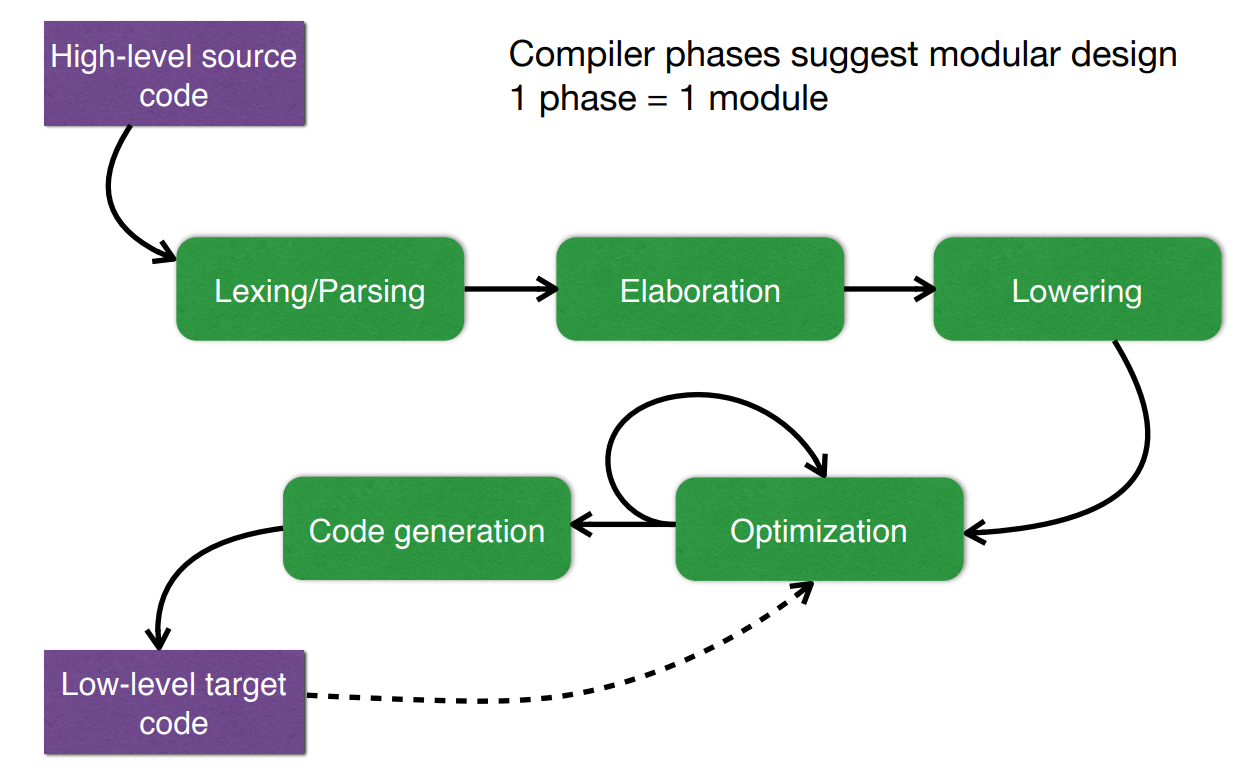
\includegraphics[scale=0.4]{assets/phases.png}
    \caption{Compiler modular phases.}
    \label{fig:phase}
\end{figure}

\begin{figure}[h]
    \centering
    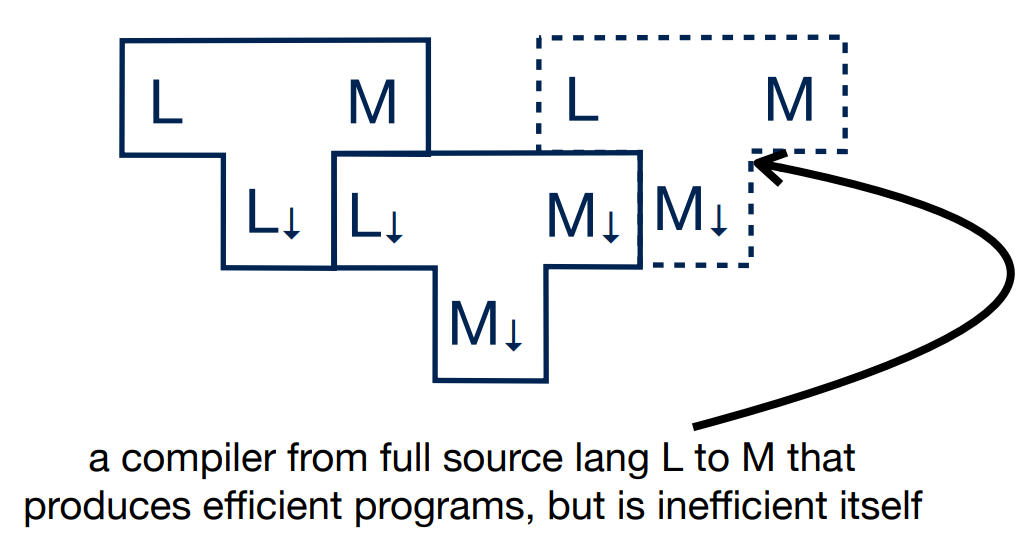
\includegraphics[scale=0.4]{assets/bootstrap_compile.png}
    \caption{Bootstrap compiling}
    \label{fig:bootstrap}
\end{figure}

\begin{itemize}
    \item \textbf{Lexing/Parsing}: String $\rightarrow_{lexing}$ Tokens $\rightarrow_{parsing}$ Abstract Syntax Tree (AST)
    \item \textbf{Elaboration}: \textit{Resolving scope }and \textit{Type checking}. Most errors found here.
    \item \textbf{Lowering}: High-level features to target-language like constructs (e.g. assembly-like). \textit{Intermediate representation}, LLVM.
    \item \textbf{Optimization}: Detect and rewrite expensive operations. Lifting invariants out of loops, parallelization.
    \item \textbf{Code generation}: fx LLVM to X86 (registers, instruction etc.)
    \item \textbf{Bootstrapping compilers}: Compile your language in your own language.
\end{itemize}

\section{Lexical}

\begin{figure}[h]
    \centering
    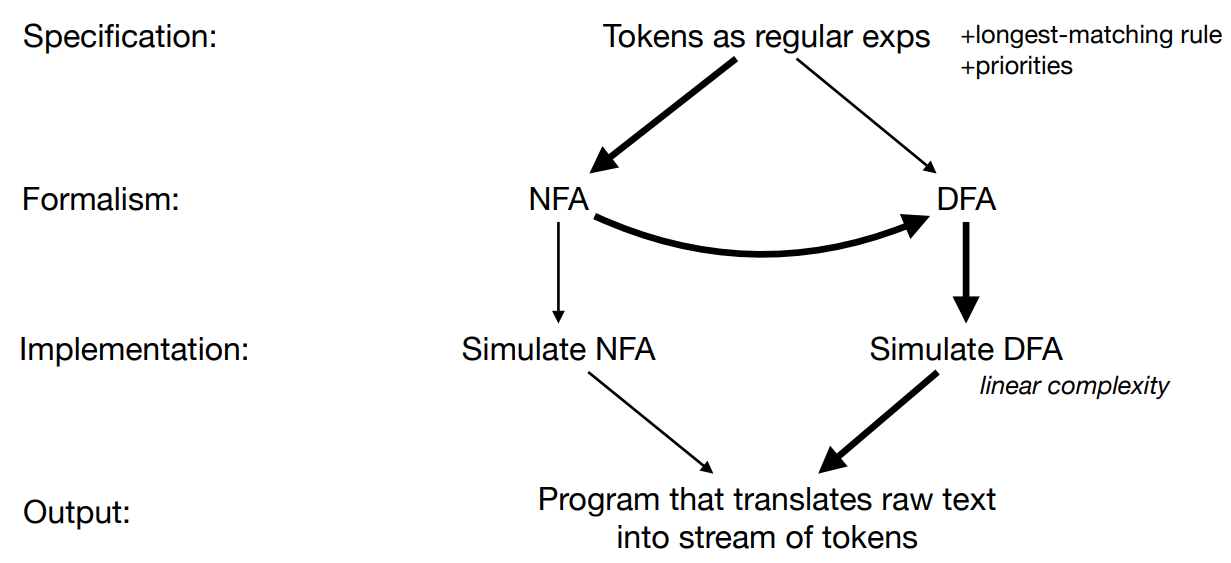
\includegraphics[scale=0.4]{assets/reg_nfa_dfa.png}
    \caption{REG to NFA to DFA}
    \label{fig:reg}
\end{figure}

\begin{itemize}
    \item Tokens: E.g. \textsc{ID}("a"), INT, IF etc. Some tokens include metadata like names in ID.
    \item Non-tokens: comments, whitespace etc.
    \item REG $\rightarrow$ NFA $\rightarrow$ (closures) DFA $\rightarrow$ Minimized DFA (more effective)
    \item REG: Handle priorities and longest matching string token wins.
    \item Ocamllex: Lexer generator
\end{itemize}

\end{document}
